\section{Augmentation des Données}
Le jeu de données obtenu suite à la séance d'enregistrement décrite dans la Section \ref{data_collection} est constitué de quatre-vingt-deux enregistrements résumés dans la Table \ref{data_collection_table}. Tel quel, ce jeu de données est insuffisant pour procéder directement à l'entraînement d'un modèle d'intelligence artificielle. En effet, pour entraîner les modèles les plus simples, il faut être en possession de suffisamment de données pour créer des jeux d'entraînement, de validation et de test. Les méthodes plus avancée relevant de l'apprentissage profond nécessitent encore plus de données d'entraînement pour être utilisées dans de bonnes conditions et offrir des résultats corrects.

Plutôt que de continuer à collecter des données, une démarche longue et peu instructive, nous avons choisi de procéder à de l'augmentation de données.

Les méthodes de \textit{data augmentation} consistent à créer de nouvelles données en altérant légèrement les données déjà présentes dans le \textit{dataset}. Lorsqu'on travaille sur des images, de nouvelles images peuvent être créer en effectuant des rotations, en rognant l'image ou en modifiant certaines propriétés (contraste, luminosité...).\\
Dans le cadre de ce projet, les données sont sous la forme de séquences numériques selon trois axes. Nou savons choisi cinq méthodes pour augmenter la quantité de données:
\begin{itemize}
    \item Renverser la séquence dans le temps
    \item Inverser l'axe correspondant à la rotation du robot
    \item Ajout de bruit
    \item Ajout d'un signal porteur
    \item Découpage des séquences
\end{itemize}

\begin{table}[]
    \begin{tabular}{|l|c|}
    \hline
    Dégradation  & \multicolumn{1}{l|}{Nombre d'enregistrements} \\ \hline
    Ralentisseur & 20                                            \\ \hline
    Racines      & 10                                            \\ \hline
    Fissure      & 20                                            \\ \hline
    Trou         & 12                                            \\ \hline
    Dalles       & 4                                             \\ \hline
    Parcours     & 16                                            \\ \hline
    \end{tabular}
    \caption{Table résumant la collecte de données}
    \label{data_collection_table}
\end{table}

Etant donnée que le robot est très réactif (l'accélération et la décélération sont similaires), nous pouvons considérer que la séquence renversée dans le temps reste représentative. (Figure \ref{data_augmentation_1})

\begin{figure}
    \center
    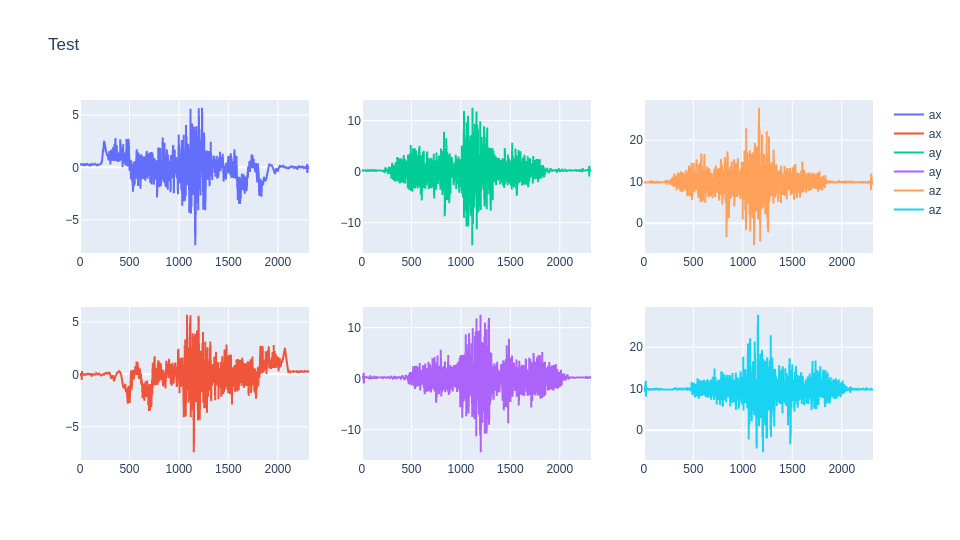
\includegraphics[scale=0.5]{img/reversed_data.png}
    \caption{Comparaison de enregistrement et de sa version modifiée (renversement du temps)}
    \label{data_augmentation_1}
\end{figure}

De la même façon, inverser la rotation du robot ne modifie pas l'enregistrement du point de vue des dégradations de la route. Les dégradations ont principalement un effet sur l'axe vertical et n'impactent pas la direction du robot donc nous pouvons prendre l'opposée des valeurs sur l'axe X. (Figure \ref{data_augmentation_2})

\begin{figure}
    \center
    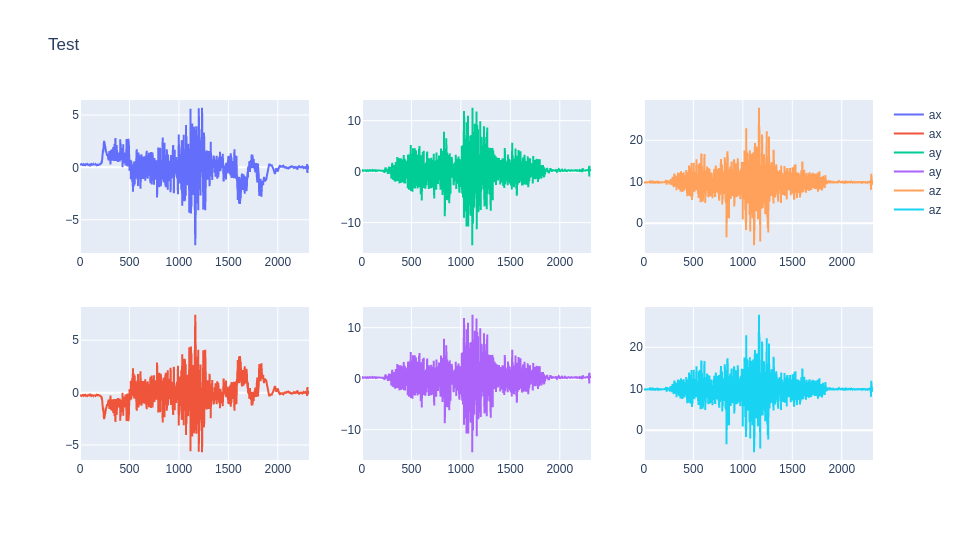
\includegraphics[scale=0.5]{img/inverted_data.png}
    \caption{Comparaison de enregistrement et de sa version modifiée (renversement d'un axe horizontal)}
    \label{data_augmentation_2}
\end{figure}

Une méthode classique pour augmenter la quantité de données consiste à ajouter du bruit. Cette méthode s'applique dans une certaine mesure aux données accélérométriques recueillies. Un faible bruit peut simuler un bitume moins lisse mais un trop gros bruit signifierait que la route est dans un mauvais état global (gravier...).

Des recherches sur internet \cite{TerryUm_ICMI2017} nous ont montré qu'il est aussi possible d'ajouter un signal porteur pour simuler un dénivelé supplémentaire. Un enregistrement de passage dans trou sur un sol horizontal peut devenir un enregistrement de passage dans un trou au cours d'une montée.

Une dernière méthode simple de \textit{data augmentation} consiste à découper les séquences dans le temps pour isoler les dégradations lors de parcours ou tout simplement pour obtenir des séquences de longueur différentes avec le passage sur la dégradation à différents moments de l'enregistrement (pas nécessaireemnt au milieu) ce qui pourrait induire un biais d'apprentissage.

Finalement, les méthodes précédentes peuvent être combinées afin de générer de nouvelles séquences artificielles.